\documentclass[border=12pt]{standalone}
\usepackage{fontspec}
\setmainfont{Helvetica}
\setsansfont{Helvetica}
\newfontfamily\arrowfont{Arial}
\renewcommand{\familydefault}{\sfdefault}
\usepackage{tikz}
\usetikzlibrary{positioning,arrows.meta,calc}
\newcommand{\hd}[1]{{\Large\bfseries #1}\\[16pt]}
\newcommand{\bx}[1]{\parbox[t][6.9cm][t]{5.3cm}{\centering #1}}
\begin{document}
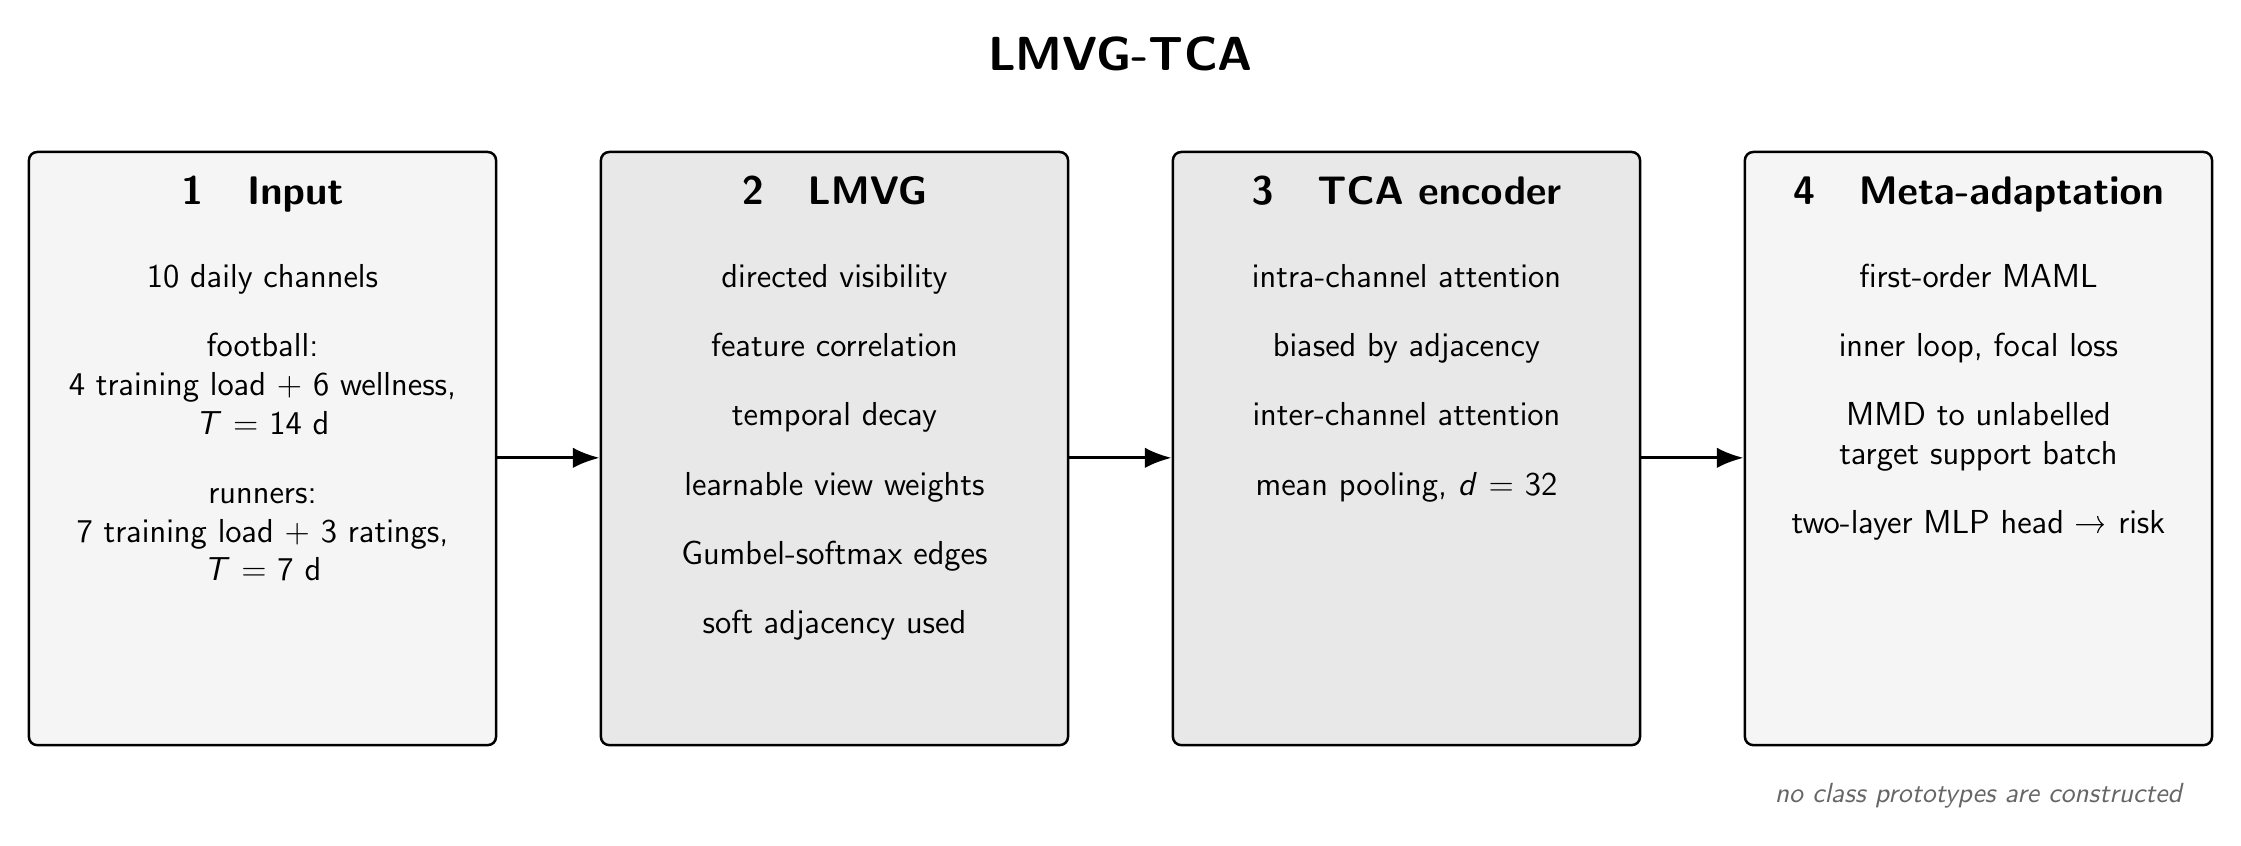
\begin{tikzpicture}[
  box/.style={draw=black,line width=0.9pt,rounded corners=3pt,inner sep=9pt,font=\large,anchor=north},
  arr/.style={-{Latex[length=3.4mm,width=2.6mm]},line width=1.1pt}]
\node[box,fill=black!4] (a) at (0,0) {\bx{\hd{1\quad Input}10 daily channels\\[11pt]football:\\4 training load + 6 wellness,\\\textit{T} = 14 d\\[11pt]runners:\\7 training load + 3 ratings,\\\textit{T} = 7 d}};
\node[box,fill=black!9,right=1.3cm of a.north east,anchor=north west] (b) {\bx{\hd{2\quad LMVG}directed visibility\\[11pt]feature correlation\\[11pt]temporal decay\\[11pt]learnable view weights\\[11pt]Gumbel-softmax edges\\[11pt]soft adjacency used}};
\node[box,fill=black!9,right=1.3cm of b.north east,anchor=north west] (c) {\bx{\hd{3\quad TCA encoder}intra-channel attention\\[11pt]biased by adjacency\\[11pt]inter-channel attention\\[11pt]mean pooling, \textit{d} = 32}};
\node[box,fill=black!4,right=1.3cm of c.north east,anchor=north west] (d) {\bx{\hd{4\quad Meta-adaptation}first-order MAML\\[11pt]inner loop, focal loss\\[11pt]MMD to unlabelled\\target support batch\\[11pt]two-layer MLP head {\arrowfont →} risk}};
\node[font=\LARGE\bfseries,above=0.9cm of $(b.north east)!0.5!(c.north west)$] {LMVG-TCA};
\node[font=\normalsize\itshape,text=black!60,below=0.35cm of d.south] {no class prototypes are constructed};
\draw[arr] ([yshift=-3.9cm]a.north east) -- ([yshift=-3.9cm]b.north west);
\draw[arr] ([yshift=-3.9cm]b.north east) -- ([yshift=-3.9cm]c.north west);
\draw[arr] ([yshift=-3.9cm]c.north east) -- ([yshift=-3.9cm]d.north west);
\end{tikzpicture}
\end{document}
